% !TEX root = ./Vorlesungsmitschrift AGLA 2.tex  
\lecture{Di 05.05. 10:15}{}
\begin{lemma}\label{teilverhaeltnis_invariant_unter_affinen_abbildungen}
    Seien \( X,Y \) affine Räume und \( f\maps X\to Y \) eine affine Abbildung, seien \( p_0,p1,p \) Punkte in \( X \), die auf einer Geraden liegen und \( f(p_0)\neq f(p_1) \). Dann gilt
    \begin{align*}
        \teilverhaeltnis{f(p_0)}{f(p_1)}{f(p)}=\teilverhaeltnis{p_0}{p_1}{p}.
    \end{align*}
\end{lemma}
\begin{proof}
    Sei \( \lambda=\teilverhaeltnis{p_0}{p_1}{p} \), also \( \vv{p_0 p}=\lambda\vv{p_0 p_1} \). Sei \( F\maps T(X)\to T(Y) \) die zu \( f \) gehörige lineare Abbildung. Wir berechnen
    \begin{align*}
        \vv{f(p_0) f(p)}\begin{aligned}[t]
            &=F(\vv{p_0 p})\\
            &=F(\lambda{p_0 p_1})\\
            &=\lambda F({p_0 p_1})\\
            &=\lambda \vv{f(p_0) f(p_1)}
        \end{aligned}
    \end{align*}
    
\end{proof}
\begin{anwendung*}[Strahlensatz]
    Sei \( X \) ein affiner Raum über \( K \), \( p_0,p_1,p_2\in X \) affin unabhängig. Sei
    \begin{align*}
        q_1&\in p_0\vee p_1,\logicspace q_1\neq p_0\\
        q_2&\in p_0\vee p_2,\logicspace q_2\neq p_0.
    \end{align*}
    Wir nehmen an, dass \( p_1\vee p_2 \) und \( q_1\vee q_2 \) parallel sind in dem Sinn, dass
    \begin{align*}
        T(p_1\vee p_2)=T(q_1\vee q_2)\text{ in }T(X).
    \end{align*}
    Dann gilt
    \begin{align*}
        \teilverhaeltnis{p_0}{p_1}{q_1}=\teilverhaeltnis{p_0}{p_2}{q_2}.
    \end{align*}
    \begin{figure}[H]
        \centering
        \includegraphics[width=0.5\linewidth]{figures/Strahlensatz}
        \label{fig:Strahlensatz}
    \end{figure}
\end{anwendung*}
\begin{proof}
    Sei \( Y \) diedurch \( p_0,p_1,p_2 \) aufgespannte Ebene. Dann gibt es ein affines Koordinatensystem \( \phi\maps K^2 \to Y \) mit \( \phi(0)=p_0, \phi(e_1)=p_1, \phi(e_2)=p_2 \).
    \begin{figure}[H]
        \centering
        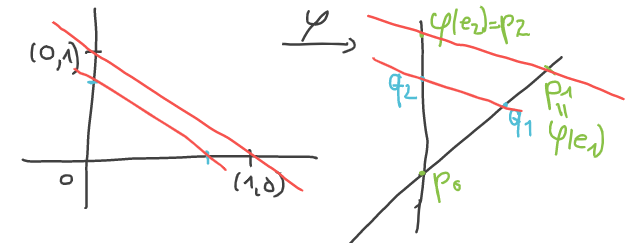
\includegraphics[width=0.5\linewidth]{figures/strahlensatz_koordinatensystem}
        \label{fig:strahlensatz_koordinatensystem}
    \end{figure}
    Sei
    \begin{align*}
        (\lambda,0)&=\inv{\phi}(q_1)\\
        (0,\mu)&=\inv{\phi}(q_2).
    \end{align*}    
    \begin{behauptung*}
        \( l_1=\inv{\phi}(q_1)\vee \inv{\phi}(q_2) \) und \( l_2=\inv{\phi}(p_1)\vee \inv{\phi}(p_2) \) sind parallel.
    \end{behauptung*}
    \minisec{Denn:}
    \begin{align*}
        T(l_1)&=K\vv{\inv{\phi}(q_1) \inv{\phi}(q_2)}\\
        T(l_2)&=K\vv{\inv{\phi}(p_1) \inv{\phi}(p_2)}.
    \end{align*}
    Es ist \( K\vv{p_1 p_2}=K\vv{q_1 q_2} \) und daher
    \begin{align*}
        \equalto{K\vv{\inv{\phi}(q_1) \inv{\phi}(q_2)}}{K \inv{\Phi}(\vv{p_1 p_2})}=\equalto{K\vv{\inv{\phi}(p_1) \inv{\phi}(p_2)}}{K\inv{\Phi}(\vv{q_1 q_2}}).
    \end{align*}
    Aus der Parallelität von \( l_1,l_2 \) folgt \( \lambda=\mu \).

    Also
    \begin{align*}
        &\rphantom{=}\teilverhaeltnis{\inv{\phi}(p_0)}{\inv{\phi}(p_1)}{\inv{\phi}(q_1)}=\lambda\\
        &=\mu=\teilverhaeltnis{\inv{\phi}(p_0)}{\inv{\phi}(p_2)}{\inv{\phi}(q_2)}
    \end{align*}
    und der Strahlensatz folgt aus \thref{teilverhaeltnis_invariant_unter_affinen_abbildungen}.
\end{proof}
\section{Affinkombinationen}
\begin{beispiel*}
    Seien \( p_0,p_1\in \reals^2 \), \( p_0\neq p_1 \). Ziel: Beschreibe den affinen Unterraum \( p_0\vee p_1 \) als Teilmenge des \( \reals^2 \). Sei \( p\in p_0\vee p_1 \). Dann \( \exists \lambda\in \reals \) mit \( \vv{p_0 p}=\lambda \vv{p_0 p_1} \) und als Vektoren im \( \reals^2 \) gilt \( p=p_0+\lambda(p_1-p_0) \). Es gilt
    \begin{align*}
        p_0 \vee p_1=\Set{(1-\lambda)p_0+\lambda p_1,\logicspace \lambda\in \reals}.
    \end{align*}
    \begin{figure}[H]
        \centering
        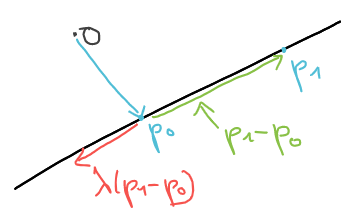
\includegraphics[width=0.5\linewidth]{figures/affine_verbindungsgerade}
        \label{fig:affine_verbindungsgerade}
    \end{figure}
    
\end{beispiel*}
\begin{frage*}
    Verallgemeinerung zu höherdimensionalen Räumen?
\end{frage*}
\begin{definition*}
    Seien \( p_0,\dotsc,p_k\in  K^n \). Wir nennen eine Linearkombination
    \begin{align*}
        \lambda_0 p_0+\lambda_1 p_1+\dotsb+\lambda_m p_m
    \end{align*}
    mit \( \lambda_i\in K \), \( 0\leq i\leq m \) eine Affinkombination oder affin falls gilt \( \lambda_0+\lambda_1+\dotsb+\lambda_m=1 \).
\end{definition*}
\begin{satz}
    Seien \( p_0,\dotsb,p_m\in K^n \). Dann gilt
    \begin{align*}
        p_0\vee \dotsb \vee p_m =\Set{\sum_{i=0}^{m}\lambda_i p_i\in K^n \logicspace \lambda_0,\dotsc,\lambda_m\in K, \sum_{i=0}^{m}\lambda_i=1}.
    \end{align*}
\end{satz}
\begin{proof}
    Sei \( Y=p_0 \vee\dotsb\vee p_m\in K^n \). Es gilt
    \begin{align*}
        T(Y)\begin{aligned}[t]
            &=\underbrace{T(p_m)}_{=0}+T(p_0\vee \dotsb \vee p_{m-1})+\underbrace{K\vv{p_0 p_m}}_{\mathclap{=T(p_0\vee p_m)}}\\
            &=K\vv{p_0 p_m}+T(p_0\vee \dotsb\vee p_{m-1})\\
            &=K\vv{p_0 p_m}+\dotsb +K\vv{p_0 p_1}\\
            &\vdots\\
            &=K\vv{p_0 p_m}+\dotsb + K\vv{p_0 p_1}\\
            &=\span(\vv{p_0 p_1}, \dotsc, \vv{p_0 p_m}).
        \end{aligned}
    \end{align*}
    Sei \( p\in K^n \). Dann ist \( p\in Y \) genau dann, wenn \texists \( \lambda_1,\dotsc,\lambda_m\in K \) mit
    \begin{align*}
        \vv{p_0 p}=\lambda_1 \vv{p_0 p_1}+\dotsb+\lambda_m\vv{p_0 p_m}.
    \end{align*}
    Im \( K^n \) gilt dann also
    \begin{align*}
        p-p_0=\lambda_1(p_1-p_0)+\dotsb + \lambda_m(p_m-p_0)
    \end{align*}
    oder 
    \begin{align*}
        p=\lambda_0 p_0+\lambda_1 p_1+\dotsb+\lambda_m p_m
    \end{align*}
    mit \( \lambda_0=1-\lambda_1-\dotsb-\lambda_m \), \dh \( \sum\limits_{i=0}^{m}\lambda_i=1 \).
\end{proof}
\section{Affine Abbildungen und Matrizen, Fixpunkte}
\begin{motivation*}
    Seien \( V,W \) \( K \)-Vektorräume, \( F\maps V\to W \) eine lineare Abbildung. Wenn wir für \( V \) und \( W \) Basen wählen, dann können wir die Abbildung \( F \) eindeutig durch eine Matrix beschreiben.
\end{motivation*}
\begin{frage*}
    Inwiefern können wir affin Abbildung zwischen affinen Räumen durch Matrizen beschreiben?
\end{frage*}
Wahl von Basen in Vektorräumen \( \leftrightarrow \) Wahl von Koordinaten in affinen Räumen. 

Seien \( X,Y \) affine Räume über \( K \), \( f\maps X\to Y \) eine affine Abbildung. Wähle affine Koordinatensysteme \( \phi\maps K^n\to X  \) und \( \psi\maps K^m\to Y \).

Wir haben das folgende kommutative Diagramm
\begin{equation*}
    \begin{tikzcd}
        K^n\arrow{r}{\phi}\arrow{d}[name=g]{g} &X\arrow{d}[name=f]{f}\\
        K^m\arrow{r}{\psi}&Y
        \arrow[to path={(f) node[midway,scale=1] {\rotatebox{90}{\(\circlearrowright\)}} (g)}]{} 
    \end{tikzcd}    
\end{equation*}
mit \( g=\inv{\psi}\circ f\circ \phi \) affin. \( g \) ist affin, also besteht eine affine Abbildung \( G\maps K^n\to K^m \) mit
\begin{align*}
    g(x)-g(0)=G(x)\quad \forall x\in K^n.
\end{align*}
\( G \) ist linear, also können wir \( G \) durch eine Matrix \( A \) ausdrücken.
\begin{align*}
    g(x)=Ax+b\quad \forall x\in K^n.
\end{align*}
mit \( b=g(0) \).
\begin{frage*}
    Wie können wir \( A \) berechnen gegeben eine affine Basis \( (p_0,\dotsc,p_n) \) von \( K^n \) und \( g(p_i) \), \( 0\leq i \leq n \)?
\end{frage*}
\begin{figure}[H]
    \centering
    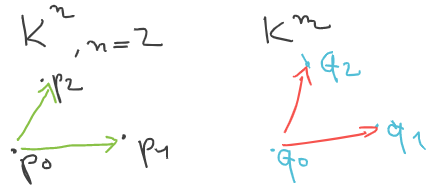
\includegraphics[width=0.5\linewidth]{figures/affine_basen_abbildung_wunsch}
    \label{fig:affine_basen_abbildung_wunsch}
\end{figure}
Wir betrachten die Matrizen \( B\in \matrices{m}{n}{K} \) bestehend aus den Spaltenvektoren \( \vv{q_0 q_1},\dotsc, \vv{q_0 q_n} \) und \( S\in \matrices{n}{n}{K} \) bestehend aus den Spaltenvektoren \( \vv{p_0 p_1}, \dotsc, \vv{p_0 p_n} \). Dann gilt \( A=B\cdot \inv{S}  \) und \( g(x)-g(p_0)=A(x-p_0) \), also \( g(x)=Ax+b \) mit \( b=g(p_0)-Ap_0 \).
\begin{bemerkung*}
    Wählen wir für \( p_0,\dotsc,pm \) die affine Basis \( 0,e_1,\dotsc, e_n \), dann \( S=\Id_{n\times n} \) und \( A=B \).
\end{bemerkung*}
\subsection*{Fixpunkte}
\begin{beispiel}
    Betrachte die affine Abbildung \( f\maps K\to K \), \( K \) ein Körper, in der Matrizendarstellung gegeben durch \( f(x)=2x+1\isittrue{=}x \).
    \begin{figure}[H]
        \centering
        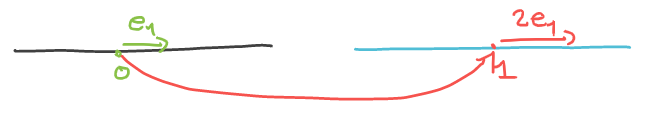
\includegraphics[width=0.5\linewidth]{figures/affiner_fixpunkt_1_d}
        \label{fig:affiner_fixpunkt_1_d}
    \end{figure}
    Dann gibt es genau ein \( x\in K \) mit \( f(x)=x \), nämlich \( x=-1 \).
\end{beispiel}
\begin{definition*}
    Sei \( X \) ein affiner Raum \( f\maps X\to X \) eine affine Abbildung. Wir nennen
    \begin{align*}
        \fixpunkte{f}\definedas \Set{x\in X|f(x)=x}
    \end{align*}
    die Menge der Fixpunkte von \( f \).
\end{definition*}
\begin{frage*}
    Welche Struktur hat \( \fixpunkte{f} \).
\end{frage*}
\begin{beispiel}
    \( X \) affiner Raum.
    \begin{align*}
        \Id\maps \begin{aligned}[t]
            X&\to X\\
            x&\mapsto x
        \end{aligned}
    \end{align*}
    dann \( \fixpunkte{\Id}=X \).
\end{beispiel}
\begin{beispiel}
    \( f\maps K^n\to K^n \), \( x\mapsto \underrelate{\isittrue{=}}{x}{\underbrace{x+p_0}} \) mit \( p_0\in K^n\setminus \zeroset \), dann \( \fixpunkte{f}=\emptyset \).
\end{beispiel}
\begin{beispiel}
    \begin{frage*}
        Was sind die Fixpunkte einer Projektion?
    \end{frage*}
    
\end{beispiel}
\begin{lemma}\label{affine_fixpunkte_sind_affiner_unterraum}
    \( \fixpunkte{f}\subseteq X \) ist ein affiner Unterraum.
\end{lemma}
\begin{proof}
    Falls \( \fixpunkte{f}=\emptyset \) dann \checkmark. Sei also \( \fixpunkte{f}\neq \emptyset \) und \( p\in \fixpunkte{f} \), \( F \) die zu \( f \) gehörig lineare Abbildung.

    Für \( x\in \fixpunkte{f} \) gilt
    \begin{align*}
        \vv{px}=\vv{f(p) f(x)}=F(\vv{px}).
    \end{align*}
    Umgekehrt folgt aus
    \begin{align*}
        \vv{px}=F(\vv{px})=\vv{p f(x)},
    \end{align*}
    dass \( x=f(x) \), also \( x\in \fixpunkte{f} \).

    Damit gilt
    \begin{align*}
        \Set{\vv{px}\in T(X)|x\in \fixpunkte{f}}=\Set{\vv{px}\in T(X)|\vv{px}=F(\vv{px})}
    \end{align*}
    und wir erkennen diese Menge als \( K \)-Untervektorraum von \( X \).
\end{proof}
\begin{frage*}
    Bestimmung von \( \fixpunkte{f} \) für eine beliebige affine Abbildung \( f\maps X\to X \)?
\end{frage*}
Nach Wahl eines Koordinatensystems können wir auf den Fall \( X=K^n \) reduzieren und annehmen, dass \( f \) in Matrizendarstellung gegeben ist.

Sei also
\begin{align*}
    f\maps \begin{aligned}[t]
        K^n&\to K^n\\
        x\mapsto &\underbrace{Ax+b}_{=x=\Id_n x}.
    \end{aligned}
\end{align*}
Dann gilt
\begin{align*}
    \fixpunkte{f}=\set{x\in K^n|(A-\explain{\text{Einheitsmatrix der Dimension \( n \):}\ \begin{pNiceMatrix}
        1 &  & 0 \\
         & \ddots &  \\
        0 &  & 1
    \end{pNiceMatrix}
    }{\Id_n})x=-b}
\end{align*}
Wir haben das Problem also reduziert auf das Lösen eines linearen Gleichungssystems.
\begin{bemerkung*}
    Daraus kann man auch \thref{affine_fixpunkte_sind_affiner_unterraum} ableiten.
\end{bemerkung*}
\begin{beispiel}\label{dilatation_beispiel}
    \begin{align*}
        f\maps \begin{aligned}[t]
            K^n&\to K^n\\
            x&\mapsto \lambda \Id_n x+b
        \end{aligned}     
    \end{align*}
    mit \( \lambda\in K \).

    Dann
    \begin{align*}
        \fixpunkte{f}=\Set{x\in K^n|(\lambda-1)x=-b}.
    \end{align*}
    Falls \( \lambda-1 \) invertierbar ist \( (\lambda\neq 1) \), gibt es genau einen Fixpunkt.
\end{beispiel}
\begin{definition*}
    Sei \( f\maps X\to X \) eine affine Abbildung mit zugehöriger linearer Abbildung \( F\maps T(X)\to T(X) \). Wir nennen \( f \) eine \emph{Dilatation} mit \emph{Faktor \( \lambda \)}, falls gilt
    \begin{align*}
        F=\lambda \cdot \Id_{T(X)}\quad \lambda\in K.
    \end{align*}
    Im Fall \( \lambda=1 \) nennen wir \( f \) eine Translation.
\end{definition*}
\begin{lemma}
    Sei \( f\maps X\to X \) eine Dilatation mit Faktor \( \lambda\neq 1 \). Dann gilt
    \begin{align*}
        \anzahl-{\fixpunkte{f}}=1.
    \end{align*}
\end{lemma}
\begin{proof}
    Nach Wahl eines Koordinatensystems reduzieren wir das Problem auf \thref{dilatation_beispiel}.    
\end{proof}

\section{Kollineationen}
Sei \( f\maps X\to X \) eine affine Abbildung eines affinen Raumes \( X \), \zb eine Affinität. Seien \( p_1,p_2,p_3\subset X \) in einer Geraden \( \ell\subseteq X \) enthalten.
\begin{figure}[H]
    \centering
    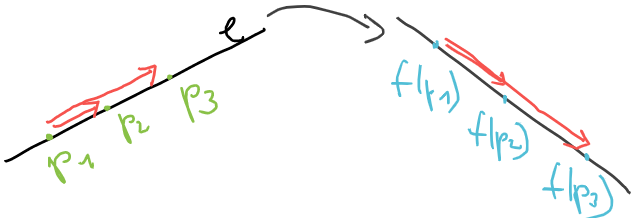
\includegraphics[width=0.5\linewidth]{figures/kollineationen_motivation}
    \label{fig:kollineationen_motivation}
\end{figure}
Dann liegen auch \( f(p_1), f(p_2),f(p_3) \) auf einer Geraden.

\begin{frage*}
    Welche bijektiven Abbildungen \( f\maps X\to X \) haben diese Eigenschaft?
\end{frage*}
\begin{definition*}
    Sei \( X \) ein affiner Raum und \( p_1,p_2,p_3\in X \). Wir nennen \( p_1,p_2,p_3 \) \emph{kollinear}, wenn \( p_1,p_2,p_3 \) auf einer Geraden \( \ell \subset X \) liegen. Wir nennen eine bijektive Abbildung \( f\maps X\to X \) eine Kollineation, falls jede Gerade \( \ell \subset X \) auf eine Gerade \( f(\ell)\subset X \) abgebildet wird.
\end{definition*}
\begin{beispiel}
    Affinitäten
\end{beispiel}
\begin{beispiel}
    Ist \( \affindim-{X}=1 \) und \( f\maps X\to X \) bijektiv, dann ist \( f \) eine Kollineation.
\end{beispiel}
\begin{beispiel}\label{kollinieationen:beispiele:komplexe_konjugation}
    Sei \( X=\complexs^2 \) als affiner Raum über \( \complexs \).
    \begin{align*}
        f\maps \begin{aligned}[t]
            \complexs^2\to \complexs^2\\
            (x,y)&\mapsto &(\explain{\text{komplexe Konjugation}}{\conj{x},\conj{y          }}).
        \end{aligned}
    \end{align*}
    Dann ist \( f \) eine Kollineation. Das Bild einer Geraden
    \begin{align*}
        (x_0,y_0)+\complexs(x_1,y_1)
    \end{align*}
    ist gegeben durch die Gerade
    \begin{align*}
        (\conj{x_0},\conj{y_0})+\complexs(\conj{x_1},\conj{y_1}),
    \end{align*}
    aber \( f \) ist \emph{keine Affinität}!
\end{beispiel}
\begin{bemerkung*}
    Die komplexe Konjugation
    \begin{align*}
        \begin{aligned}[t]
            \complexs&\to \complexs\\
            x&\mapsto \conj{x}
        \end{aligned}
    \end{align*}
    ist ein Automorphismus von dem Körper \( \complexs \).
\end{bemerkung*}